\documentclass[../ASSD_TP2.tex]{subfiles}
\begin{document}

\section{Síntesis mediante modulación de frecuencia}

\subsection{Introducción}

A la hora de modelizar instrumentos musicales a través de algoritmos
matemáticos, distinguimos dos grandes categorías: modelos de señales
y modelos físicos. Los modelos de señales buscan reconstruir el sonido
que se percibe sin analizar la fuente específica que provoca el sonido,
mientras que los modelos físicos buscan simular el comportamiento
de la fuente que emite dicho sonido. 

\begin{figure}[H]
\centering{}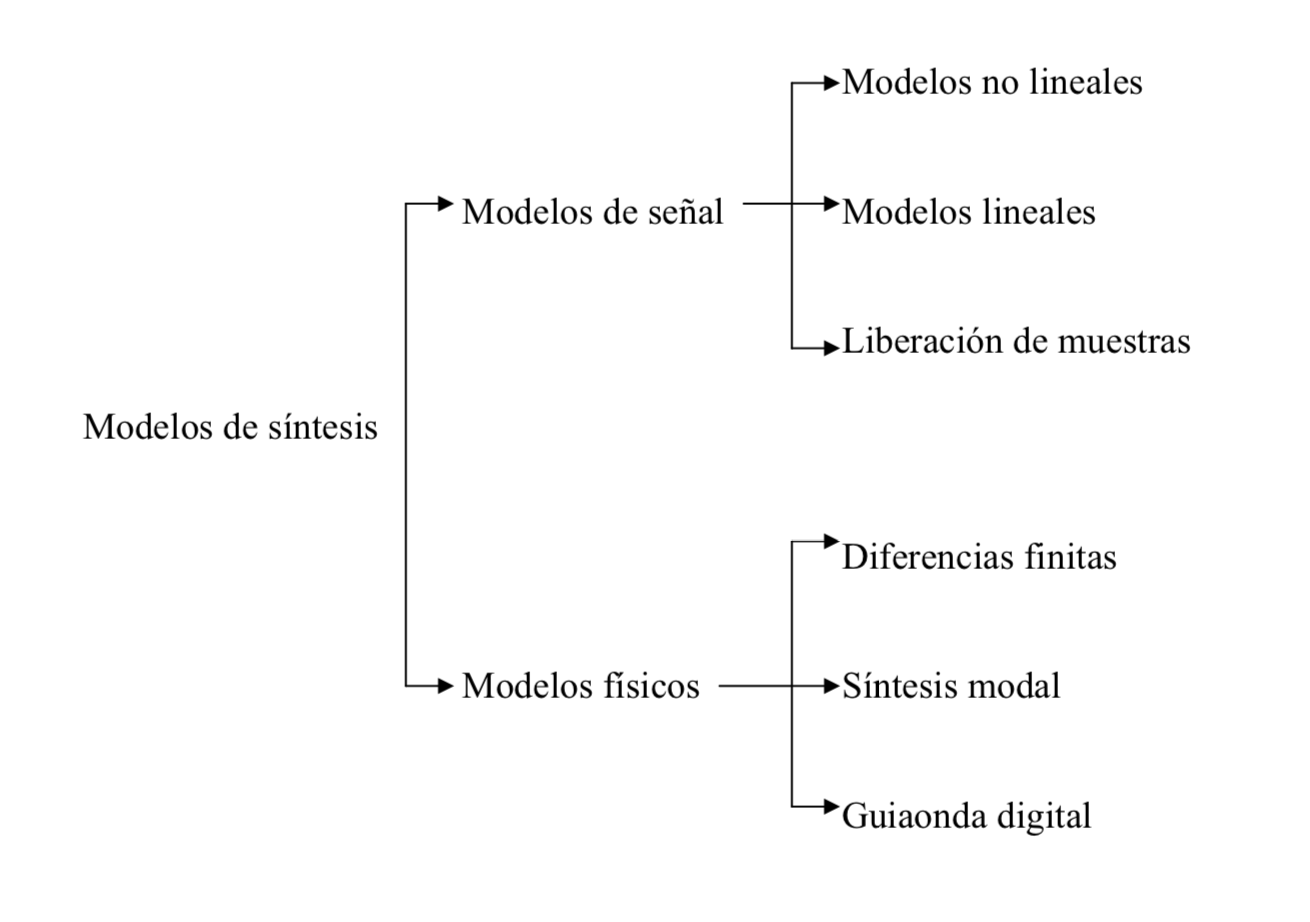
\includegraphics[scale=0.5]{imagenes/esquema}\caption{Esquema de los distintos modelos de algoritmos.}
\end{figure}

Dentro de los modelos de señal, podemos ver tres subconjuntos: modelos
lineales, no lineales y liberación de muestras. En la sección de los
métodos no lineales podemos distinguir distintos métodos de síntesis,
a saber: de síntesis FM, síntesis AFM, síntesis DFM y síntesis PD
entre varios métodos. En este trabajo práctico, nos vamos a centrar
en la síntesis de FM.

\subsection{Síntesis de FM}

El método de síntesis de FM fue presentado por la marca de teclados
Yamaha en 1980, basándose en los estudios de John Chowning sobre la
teoría FM de radiofrecuencia a la síntesis de audio. La síntesis FM
está basada, como su propio nombre indica, en la modulación en frecuencia.
La frecuencia de una onda determinada se modula por otra onda de distinta
frecuencia. El resultado contiene elementos de ambas frecuencias junto
con nuevos armónicos relacionados matemáticamente con las frecuencias
originales. Se puede demostrar teóricamente que cualquier sonido,
por complejo que sea, puede ser modelado mediante una serie de modulaciones
en frecuencia de ondas senoidales.

\subsubsection{Análisis matemático}

La ecuación general de una señal FM es la siguiente:
\begin{center}
{\large{}$\begin{cases}
y(t)=A(t)\text{·}cos(\Phi(t))\\
\Phi(t)=2\pi f_{c}t+I(t)\cdot cos(2\pi f_{m}t+\phi_{m})+\phi_{c}
\end{cases}$}{\large\par}
\par\end{center}

donde A(t) y $\Phi(t)$ son la amplitud y fase de la señal (ambas
variantes en el tiempo). Si combinamos ambas ecuaciones, asumiendo
ademas que para nuestro caso el desplazamiento de fase es de $-\frac{\pi}{2}$,
obtenemos la siguiente expresión:
\begin{center}
{\large{}$x(t)=A(t)\cdot sen(2\pi f_{c}t+I(t)\text{·}sen(2\pi f_{m}t))$}{\large\par}
\par\end{center}

Para sintetizar los distintos sonidos, basta con elegir adecuadamente
A(t) e I(t), y proporcionar una adecuada relación entre $f_{c}$ y
$f_{m}$. La función de I(t), denominada envolvente del índice de
modulación, es la de determinar el contenido armónico del sonido.
Si derivamos la fase respecto del tiempo, podemos obtener la frecuencia
instantanea 
\begin{center}
{\large{}$f_{i}=f_{c}-I(t)\cdot f_{m}sin(2\pi f_{m}t+\phi_{m})+\frac{1}{2\pi}\frac{dI(t)}{dt}\cdot cos(2\pi f_{m}t+\phi_{m})$}{\large\par}
\par\end{center}

con esa expresión, podemos ver que la relación precisa del índice
de modulación I(t), podemos lograr que la función cambie la totalidad
de sus contenidos armónicos. Normalmente tanto A(t) como I(t) suelen
ser constantes la mayor parte del tiempo y dejan de serlo normalmente
hacia el comienzo o final del sonido, para así tener en cuenta efectos
transitorios como consecuencia del ataque de tecla. Las bandas laterales
poseerán armónicos parciales a las frecuencias $f_{c}\pm nf_{m}$.
Si $f_{c}$ y $f_{m}$ son ambos racionales, en una relación 1:N,
el espectro resultante será armónico pero sin incluir los parciales
que sean múltiplos de N. Esta propiedad es muy útil para sintetizar
instrumentos de embocadura cilíndrica como el clarinete, los cuales
se caracterizan por incluir en el espectro sólo los armónicos impares
del tono fundamental. Si por el contrario $f_{c}$ y $f_{m}$ son
irracionales entonces el espectro resultante será inarmónico y por
lo tanto, se traduce una amplia paleta de timbres brillantes y vibrantes,
incluyendo tañidos de campana y similares.

La amplitud de cada parcial $f_{c}\pm nf_{m}$ es $J_{n}(I)$ donde
$J_{n}$ es la función de Bessel de orden n, de modo que el espectro
puede describirse analíticamente por:
\begin{center}
{\Large{}$Y(f)=A_{c}\cdot\sum_{n=-\infty}^{+\infty}J_{n}(I)\cdot\delta(f_{c}\pm nf_{m})$}{\Large\par}
\par\end{center}

Si aplicamos la transformada inversa de fourier, podemos escribir
la función de la siguiente manera:
\begin{center}
{\Large{}$y(t)=A_{c}\text{·}\sum_{n=-\infty}^{+\infty}J_{n}(I)\text{·}sin(/\omega_{c}\pm n\omega_{m})\cdot t)$}{\Large\par}
\par\end{center}

Podemos ver como, para I =0, es decir sin modulación, la portadora
tiene toda la energía y no hay parciales. Conforme I aumenta, la portadora
pierde fuerza y aumenta la energía de los parciales. Es posible estimar
la cantidad de parciales que serán audibles para un valor dado de
I es I +1, donde I se redondea al entero más cercano. Para generalizar,
podemos decir que a medida que I aumenta, mayor cantidad de frecuencias
serán audibles.

\subsection{Síntesis del clarinete}

Aplicando lo explicado anteriormente, para sintetizar el sonido de
un clarinete, basta con elegir adecuadamente sus funciones A(t) e
I(t) y determinar la relación entre las frecuencias de la señal modulada
y de la portadora.

Para el clarinete notamos que la mejor relación entre las frecuencias
modulada y portadora es $\frac{f_{c}}{f_{m}}=\frac{3}{1}$. 

La función A(t) es un poco más compleja. Si la dividimos en tres partes,
podemos distinguir que la primera parte, más conocida como ataque,
tiene forma de exponencial creciente. La segunda parte, conocida como
sostén, es de un valor constante; y la tercera parte, conocida como
soltar (release), es una exponencial decreciente. Esa combinación
de funciones nos otorga la mejor A(t) posible para sintetizar un clarinete.
Variando los parámetros de la exponencial y el valor de $A_{0}$ obtenemos
distintos tipos de clarinetes.

La función I(t) por el contrario posee dos partes: la primera una
exponencial creciente, y la segunda posee un valor constante $I_{0}$.

La frecuencia fundamental resultante, queda dada por el máximo común
divisor entre la frecuencia modulada y la portadora.

Podemos ver la forma de la señal y su respectivo espectro en la siguiente
figura:

\begin{figure}[H]

\begin{centering}
\includegraphics[scale=0.75]{\string"imagenes/clarinete onda\string".png}
\par\end{centering}
\begin{centering}
\includegraphics[scale=0.75]{\string"imagenes/espectrograma clarinetes\string".png}\caption{Gráfico en el tiempo y espectrograma del sonido generado por el clarinete.}
\par\end{centering}
\end{figure}


\subsection{Síntesis de la campana}

Para lograr el sonido que emite una campana, basta con establecer
una relación de 5:7 entre frecuencias portadora y modulada. Las funciones
A(t) e I(t) tienen la misma forma de exponencial negativa de la siguiente
manera:

$A(t)=I(t)=C\cdot e^{-t/\tau}$ 

donde C es la $A_{0}$ o $I_{0}$ según el caso y $\tau$ es el parámetro
que controla el tiempo de decaimiento. A distintos $A_{0}$, $I_{0}$
y $\tau$se obtienen distintos sonidos de campanas.

La frecuencia fundamental del sonido de la campana es $f_{c}/5$.

A continuación observamos el diagrama en tiempo y espectrograma de
la campana:

\begin{figure}[H]
\begin{centering}
\includegraphics[scale=0.75]{\string"imagenes/campana onda\string".png}
\par\end{centering}
\centering{}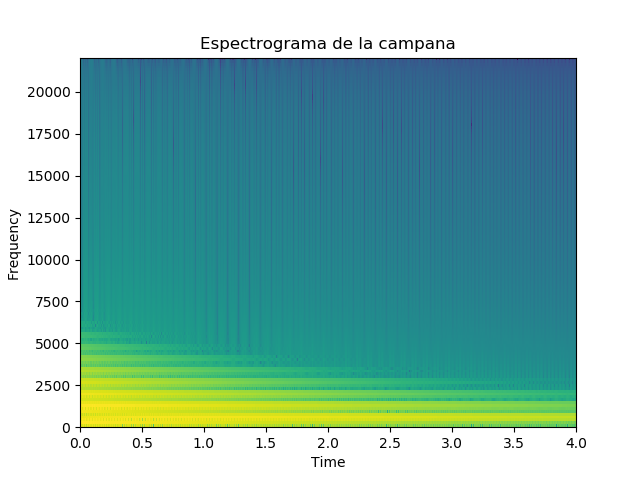
\includegraphics[scale=0.75]{imagenes/Figure_1}\caption{Gráfico en el tiempo y espectrograma del sonido generado por la campana}
\end{figure}


\subsection{Síntesis de otros instrumentos}

A partir de los dos instrumentos previamente explicados, cambiando
sus parámetros y/o su rango de operación en frecuencias, es posible
sintetizar otros instrumentos de viento. Sin embargo, el más llamativo
de todos es el que se logra cuando la relación entre las frecuencias
modulada y portadora del clarinete es de 2:3. Con esa configuración,
es posible lograr el efecto de un violín. El espectrograma resultante
es el siguiente:

\begin{figure}[H]

\begin{centering}
\includegraphics[scale=0.75]{\string"imagenes/espectograma violin\string".png}\caption{Gráfico en el tiempo y espectrograma del sonido generado por el violín}
\par\end{centering}
\end{figure}


\end{document}
